% !TEX TS-program = pdflatex
% !TEX encoding = UTF-8 Unicode

% This file is a template using the "beamer" package to create slides for a talk or presentation
% - Giving a talk on some subject.
% - The talk is between 15min and 45min long.
% - Style is ornate.

% MODIFIED by Jonathan Kew, 2008-07-06
% The header comments and encoding in this file were modified for inclusion with TeXworks.
% The content is otherwise unchanged from the original distributed with the beamer package.

\documentclass{beamer}


% Copyright 2004 by Till Tantau <tantau@users.sourceforge.net>.
%
% In principle, this file can be redistributed and/or modified under
% the terms of the GNU Public License, version 2.
%
% However, this file is supposed to be a template to be modified
% for your own needs. For this reason, if you use this file as a
% template and not specifically distribute it as part of a another
% package/program, I grant the extra permission to freely copy and
% modify this file as you see fit and even to delete this copyright
% notice.


\mode<presentation>
{
\usetheme{Warsaw}
\usefonttheme[onlylarge]{structurebold}
\usecolortheme{seagull}
\setbeamerfont*{frametitle}{size=\normalsize,series=\bfseries}
\setbeamertemplate{navigation symbols}{\insertframenumber/\inserttotalframenumber}{}
% or ...

\setbeamercovered{transparent}
% or whatever (possibly just delete it)
}




\usepackage[english]{babel}
% or whatever
\usepackage{kotex}
\usepackage{tabularx}
\usepackage{colortbl}
\usepackage{multirow}
\usepackage{booktabs}
\usepackage[utf8]{inputenc}
\usepackage{import}

% or whatever

\usepackage{times}
\usepackage[T1]{fontenc}
%\setbeamertemplate{itemize items}[default]
\setbeamertemplate{itemize item}{$\bullet$}
\setbeamertemplate{itemize subitem}{$\circ$}
\setbeamertemplate{itemize subsubitem}{$\cdot$}

\setbeamertemplate{itemize/enumerate body begin}{\footnotesize}
\setbeamertemplate{itemize/enumerate subbody begin}{\scriptsize}
\setbeamertemplate{itemize/enumerate subsubbody begin}{\scriptsize}

% huge
% large
% normalsize
% small
% footnotesize
% scriptsize
% tiny


\setlength{\leftmargin}{5pt}
\setlength{\leftmargini}{5pt}
\setlength{\leftmarginii}{5pt}
\setlength{\leftmarginiii}{5pt}


% Or whatever. Note that the encoding and the font should match. If T1
% does not look nice, try deleting the line with the fontenc.

\title[WebOS 2.0 QA spec \alert{LGE CONFIDENTIAL}] % (optional, use only with long paper titles)
{LGSE QA Test Manual Ver.15}

\subtitle
{for H15/M14+ - WebOS 2.0} % (optional)


\author[Kichul Kim, Bong-Jin Lee] % (optional, use only with lots of authors)
{Kichul Kim (kichul.kim@lge.com)\\Bong-Jin Lee (bongjin.lee@lge.com)}
% - Use the \inst{?} command only if the authors have different
%   affiliation.

\institute[IPT team, SIC lab., LG Electronics] % (optional, but mostly needed)
{
  IPT team, SIC lab., LG Electronics \\
  Release Link: (http://collab.lge.com/main/x/jLbjCQ)
  }
% - Use the \inst command only if there are several affiliations.
% - Keep it simple, no one is interested in your street address.

\date[Short Occasion] % (optional)
{\today\\ \alert{LGE CONFIDENTIAL}}

\subject{Talks}
% This is only inserted into the PDF information catalog. Can be left
% out.



% If you have a file called "university-logo-filename.xxx", where xxx
% is a graphic format that can be processed by latex or pdflatex,
% resp., then you can add a logo as follows:

% \pgfdeclareimage[height=0.5cm]{university-logo}{university-logo-filename}
% \logo{\pgfuseimage{university-logo}}



% Delete this, if you do not want the table of contents to pop up at
% the beginning of each subsection:
\AtBeginSubsection[]
{
  \begin{frame}<beamer>{Outline}
    \tableofcontents[currentsection,currentsubsection]
  \end{frame}
}


%%%%%%%%%%%%%%%%%%%%%%%%%%%%%%%%%%%%%%%%%%%%%%%%%%%%%%%%%%%%%%%%%%%%%%%%
\begin{document}
\begin{frame}
  \titlepage
\end{frame}


%%%%%%%%%%%%%%%%%%%%%%%%%%%%%%%%%%%%%%%%%%%%%%%%%%%%%%%%%%%%%%%%%%%%%%%%
\begin{frame}[t]{Test Spec. 사용 및 관리}

 \begin{itemize}
 \item Test Spec 변경의 원인은 아래와 같습니다.
 	\begin{itemize}
	\item 기능의 특성상 각 기능의 parameter 값이 튜닝 후 변경되면, 특성들이 변경됩니다.
	\item 이 때문에, parameter 변경을 하게 되면 Spec도 변경되게 됩니다.
	\end{itemize}
\end{itemize}

 \begin{itemize}
 \item Test Spec 사용
 	\begin{itemize}
 	\item Test Spec은 현재 기준으로 가장 최종 Spec을 적용하여 사용하시면 됩니다.
	\end{itemize}
\end{itemize}

 \begin{itemize}
 \item Test Spec 관리
 	\begin{itemize}
 	\item parameter 값을 튜닝 및 관리하는 TV 음팀과 SIC 연구소 IPT팀에서 Spec 배포 및 관리하며, 최종 버전 문서만 관리 대상입니다.
	\end{itemize}
\end{itemize}

\end{frame}

%%%%%%%%%%%%%%%%%%%%%%%%%%%%%%%%%%%%%%%%%%%%%%%%%%%%%%%%%%%%%%%%%%%%%%%%
\begin{frame}[t]{History}
\begin{itemize}
\begin{scriptsize}
\item 2014.07.26\_Ver.1 Init
\item 2014.07.29\_Ver.2 2spk Smart Sound (home, store), 3D Sound Zooming 수정
\item 2014.08.22\_Ver.3 4.2spk (UF95) 모델 추가
\item 2014.08.28\_Ver.4 4.2spk Game, 3D Sound Zooming 스펙 변경
\item 2014.09.03\_Ver.5 LF63 Smart Sound, 3D Sound Zooming, Game, News, Music, Sports, Surround 스펙 변경 / Punk, Pagode, Sertawego 스펙 추가
\item 2014.09.15\_Ver.6 UF95 Smart Sound, 3D Sound Zooming, Game, News, Music, Sports, Surround 스펙 변경
\item 2014.09.19\_Ver.7 UF95 Smart Sound, 3D Sound Zooming, Cinema, Game, News, Sports, Surround 스펙 변경 / High Resolution 스펙 추가
\item 2014.10.24\_Ver.8 UF85 모델 추가
\item 2014.11.06\_Ver.9 EG96 모델 추가 / UF85 sports, game, cinema 스펙 변경
\item 2014.11.20\_Ver.10 LF63 StandType 스펙 변경
\item 2014.12.02\_Ver.11 LF63/UF85/UF95 StandType, news, music 스펙 변경, LF63 game 스펙 변경
\item 2014.12.11\_Ver.12 UF85 Game 스펙 변경, 3DSZ 스펙 수정
\item 2015.01.08\_Ver.13 EG96 Cinema Store, Sports Store 스펙 변경 / Game Store, 3DSZ Store 제거 / Game 스펙 변경
\item 2015.01.08\_Ver.14 EG96 Cinema Store, Sports Store 스펙 변경
\item 2015.01.29\_Ver.15 UF86, UF83, UF77, UG87, UG73, EG92, EF95 모델 추가

\end{scriptsize}
\end{itemize}
\end{frame}


%%%%%%%%%%%%%%%%%%%%%%%%%%%%%%%%%%%%%%%%%%%%%%%%%%%%%%%%%%%%%%%%%%%%%%%%
\begin{frame}{}
\tableofcontents
\huge Audio Precision 설정 방법\\
\end{frame}



%%%%%%%%%%%%%%%%%%%%%%%%%%%%%%%%%%%%%%%%%%%%%%%%%%%%%%%%%%%%%%%%%%%%%%%%
\begin{frame}[t]{Signal Path Setting}
\begin{itemize}
\item 스피커앰프의 출력을 8옴 1\% Dummy 저항을 거쳐서 Audio Precision에 입력으로 연결합니다.
\item 테스트 신호는 Audio Precision에서 재생하는 사운드로 HDMI 혹은 unbalaced (RCA)를 이용합니다.
\item Project -> Signal Path Setup -> Level을 활성화 합니다.
	\begin{itemize}
	\item Sampling rate: 48kHz, Bit depth: 16bits
	\item Waveform: sine, Frequency: 1kHz, Level: -12dBFS (25\%FS, 500mVrms)
	\item 특별한 언급이 없는 한, 채널 L/R은 모두 같은 크기, 같은 위상의 신호를 넣어야 합니다.
	\end{itemize}
\end{itemize}

\begin{figure}[r]
	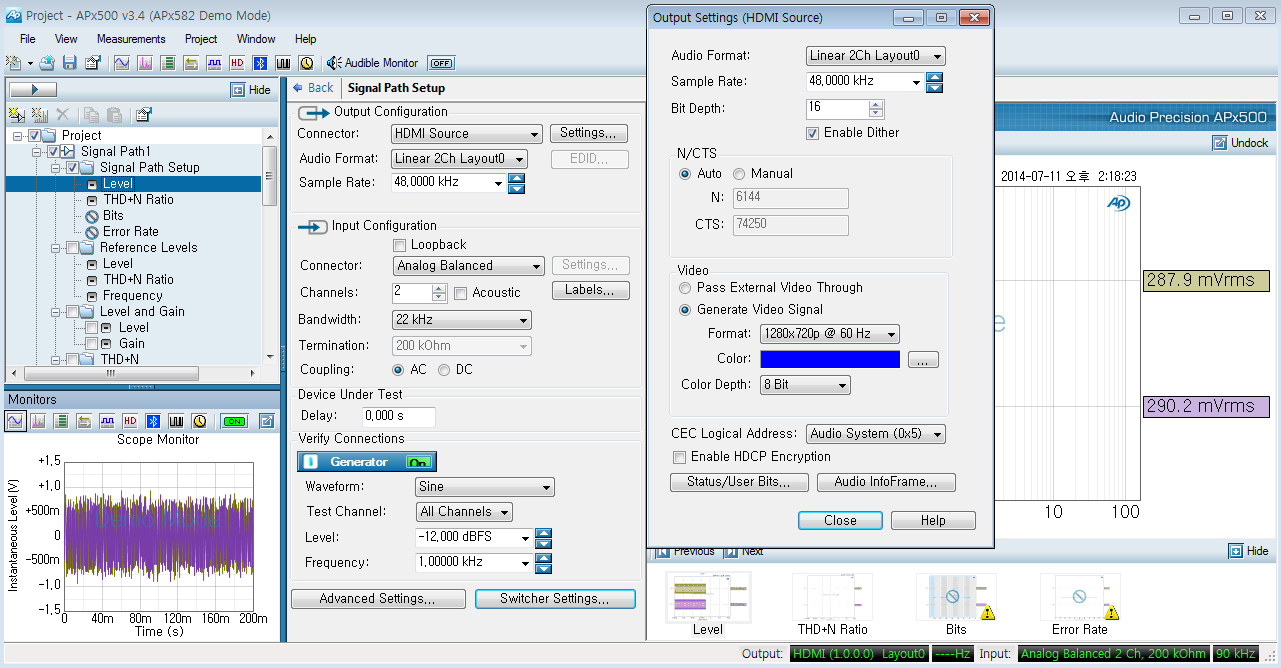
\includegraphics[height=0.4\textwidth]{figure/apsetting/signalPath.png}
\end{figure}
\end{frame}



%%%%%%%%%%%%%%%%%%%%%%%%%%%%%%%%%%%%%%%%%%%%%%%%%%%%%%%%%%%%%%%%%%%%%%%%
\begin{frame}[t]{THD+N Check}
\begin{itemize}
\item 테스트 신호는 Audio Precision에서 재생하는 사운드로 HDMI 혹은 unbalaced (RCA)를 이용합니다.
\item Project -> Signal Path Setup -> THD+N Ratio를 활성화 합니다.
	\begin{itemize}
	\item Waveform: sine, Level: 0dBFS (100\%FS, 2Vrms)
	\item 스펙항목의 Frequency를 입력 합니다.
	\end{itemize}
\end{itemize}

\begin{figure}[b]
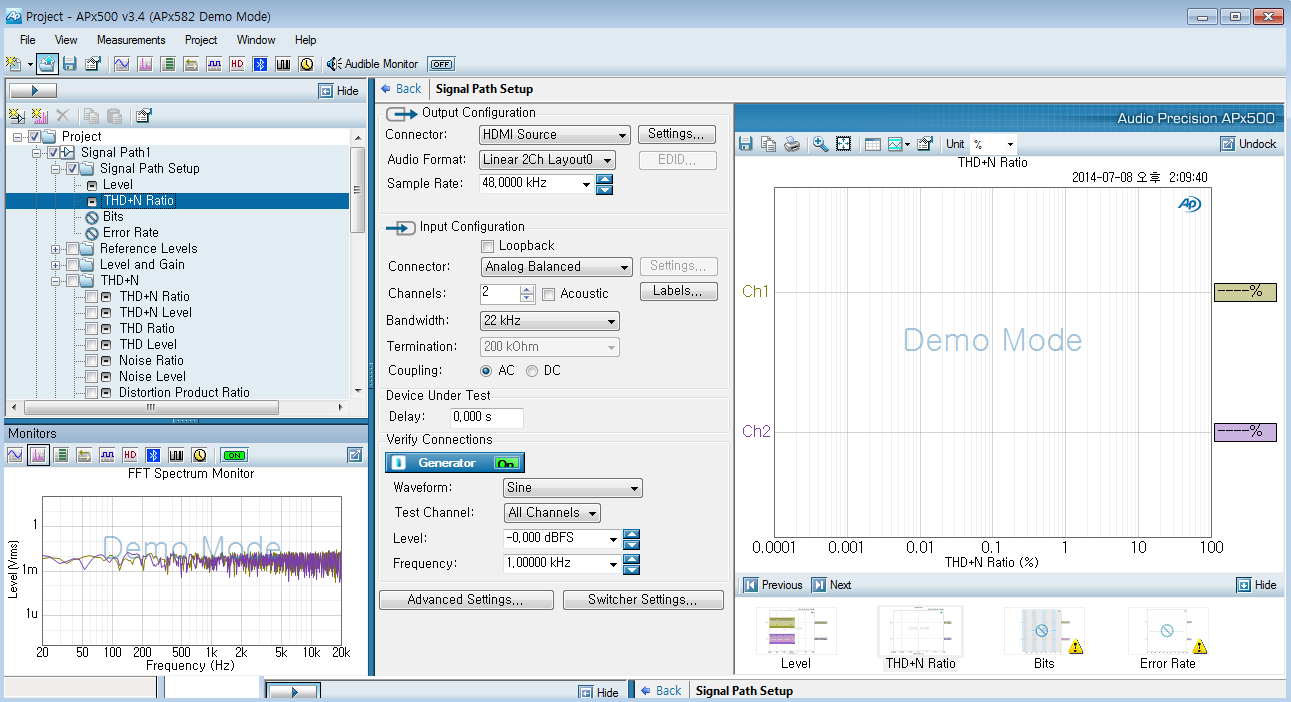
\includegraphics[height=0.4\textwidth]{figure/apsetting/thdn.png}
\end{figure}

\end{frame}


%%%%%%%%%%%%%%%%%%%%%%%%%%%%%%%%%%%%%%%%%%%%%%%%%%%%%%%%%%%%%%%%%%%%%%%%
\begin{frame}[t]{Interchannel Phase Check}
\begin{itemize}
\item 테스트 신호는 Audio Precision에서 재생하는 사운드로 HDMI 혹은 unbalaced (RCA)를 이용합니다.
\item Project -> Interchannel Phase를 활성화 합니다.
	\begin{itemize}
	\item Waveform: sine, Level: -12dBFS (25\%FS, 0.5Vrms)
	\item Ref Channel: Ch1, Meter Range: -180 -> 180 deg
	\item 스펙항목의 Frequency를 입력 합니다.
	\end{itemize}
\end{itemize}


\begin{figure}[b]
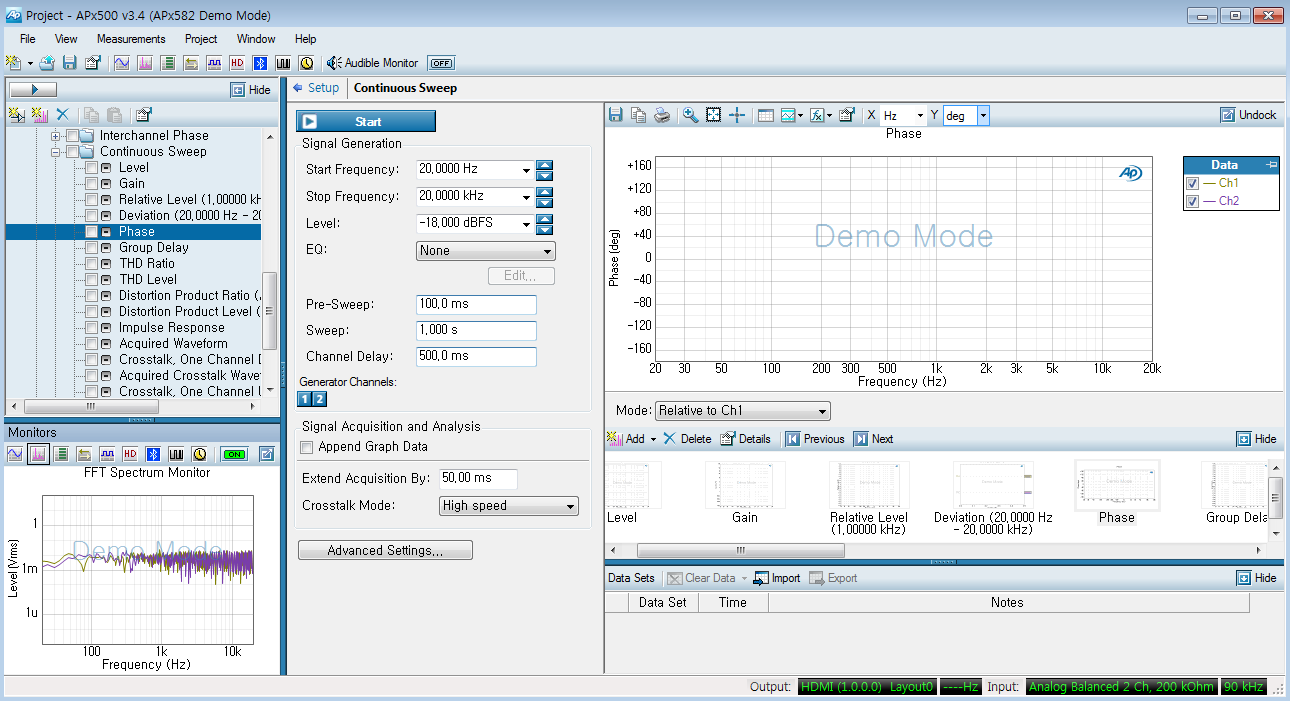
\includegraphics[height=0.4\textwidth]{figure/apsetting/interchannelPhase.png}
\end{figure}

\end{frame}

%%%%%%%%%%%%%%%%%%%%%%%%%%%%%%%%%%%%%%%%%%%%%%%%%%%%%%%%%%%%%%%%%%%%%%%%
\begin{frame}[t]{Frequency Response Check}
\begin{itemize}
\item 테스트 신호는 Audio Precision에서 재생하는 사운드로 HDMI 혹은 unbalaced (RCA)를 이용합니다.
\item Project -> Frequency Response -> Level을 활성화 합니다.
	\begin{itemize}
	\item Start Frequency: 20Hz, Stop Frequency: 20kHz
	\item Level: -12dBFS (25\%FS, 500mVrms)
	\item Pre-Sweep: 100ms, Sweep: 3s
	\end{itemize}
\item 기능이 off일 때를 기준 (ref)으로 하고, on일 때의 출력레벨 차이값을 측정합니다.
\end{itemize}

\begin{figure}[r]
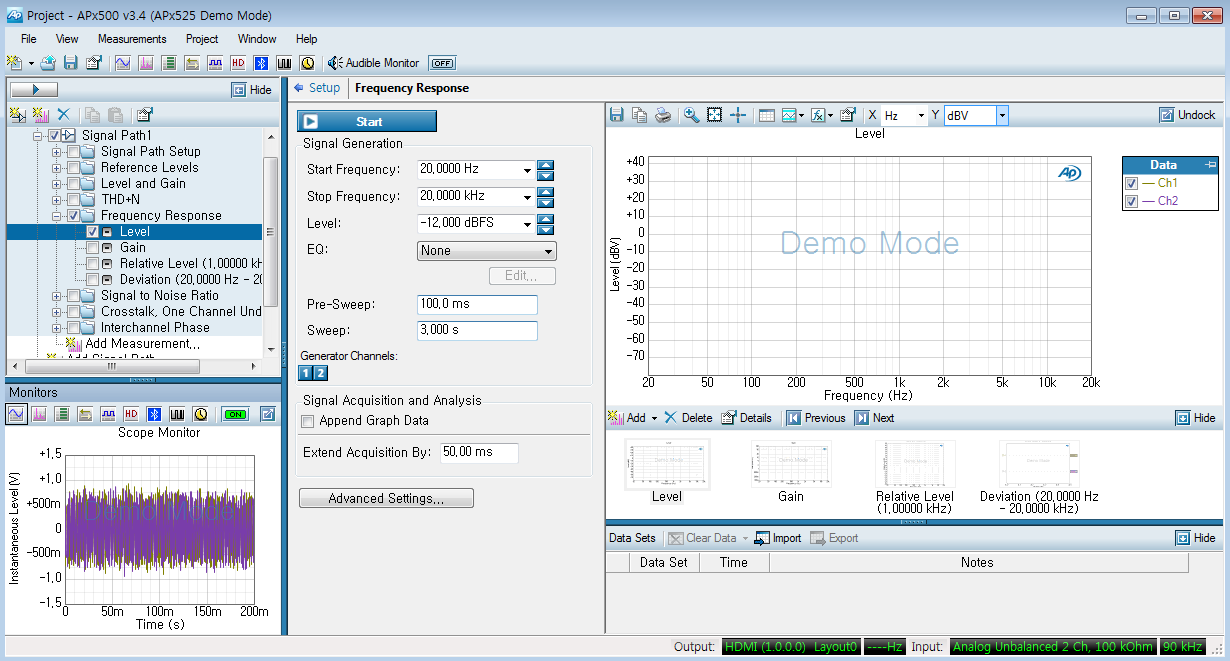
\includegraphics[height=0.4\textwidth]{figure/apsetting/frequencyResponse.png}
\end{figure}

\end{frame}


%%%%%%%%%%%%%%%%%%%%%%%%%%%%%%%%%%%%%%%%%%%%%%%%%%%%%%%%%%%%%%%%%%%%%%%%
\begin{frame}[t]{Level Check}
\begin{itemize}
\item 테스트 신호는 Audio Precision에서 재생하는 사운드로 HDMI 혹은 unbalaced (RCA)를 이용합니다.
\item Project -> Signal Path Setup -> Level을 활성화 합니다.
	\begin{itemize}
	\item Waveform: sine, Level: -12dBFS (25\%FS, 500mVrms)
	\item 스펙항목의 Frequency를 입력 합니다.
	\end{itemize}
\item 기능이 off일 때를 기준 (ref)으로 하고, on일 때의 출력레벨 차이값을 측정합니다.
\end{itemize}

\begin{figure}[r]
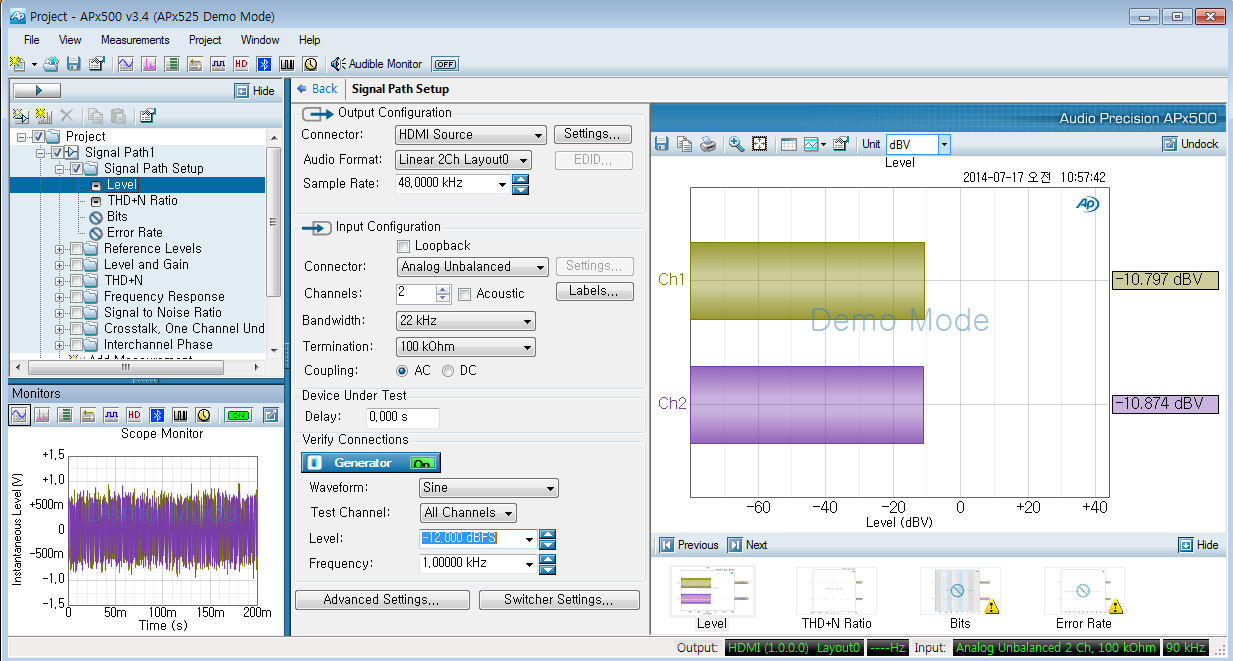
\includegraphics[height=0.4\textwidth]{figure/apsetting/level.png}
\end{figure}

\end{frame}

%%%%%%%%%%%%%%%%%%%%%%%%%%%%%%%%%%%%%%%%%%%%%%%%%%%%%%%%%%%%%%%%%%%%%%%%
\begin{frame}[t]{Antiphase Level Check}
\begin{itemize}
\item 테스트 신호는 Audio Precision에서 재생하는 사운드로 HDMI 혹은 unbalaced (RCA)를 이용합니다.
\item Project -> Signal Path Setup -> Level을 활성화 합니다.
	\begin{itemize}
	\item Waveform: split phase, Level: -12dBFS (25\%FS, 500mVrms), Phase B: 180 deg
	\item 스펙항목의 Frequency를 입력 합니다.
	\end{itemize}
\item 기능이 off일 때를 기준 (ref)으로 하고, on일 때의 출력레벨 차이값을 측정합니다.
\end{itemize}

\begin{figure}[r]
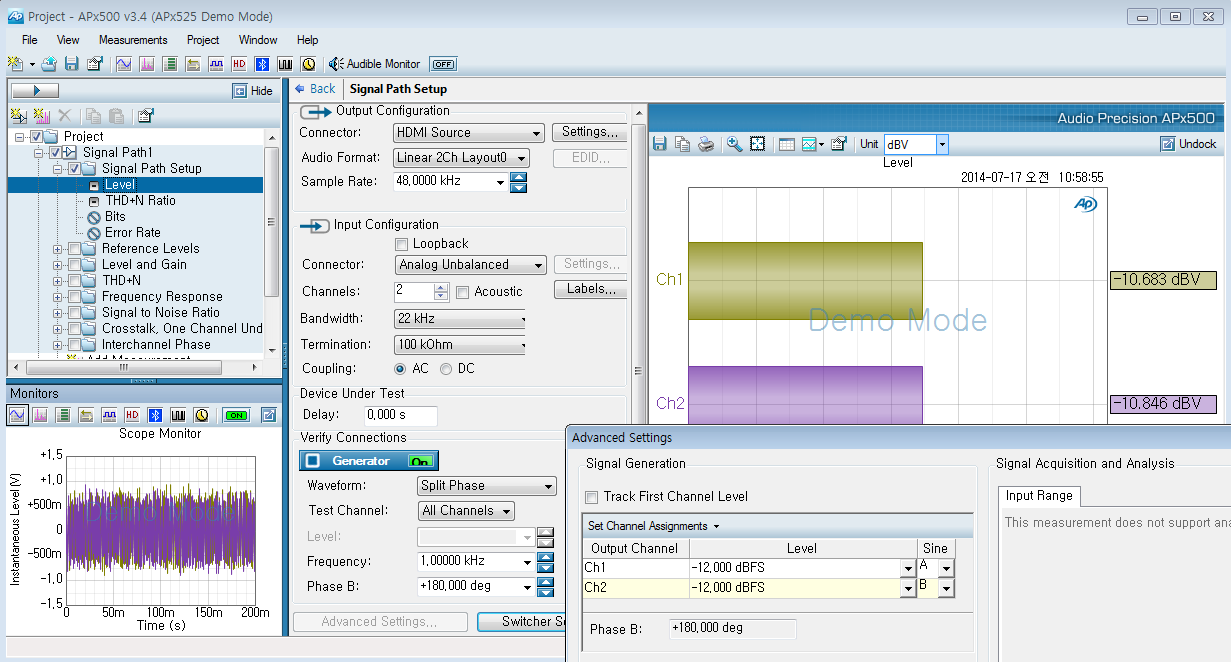
\includegraphics[height=0.4\textwidth]{figure/apsetting/antiphaseLevel.png}
\end{figure}
\end{frame}


%%%%%%%%%%%%%%%%%%%%%%%%%%%%%%%%%%%%%%%%%%%%%%%%%%%%%%%%%%%%%%%%%%%%%%%%
\begin{frame}[t]{Autovolume Level Check}
\begin{itemize}
\item 테스트 신호는 Audio Precision에서 재생하는 사운드로 HDMI 혹은 USB 입력을 이용합니다.
\item Project -> Signal Path Setup -> Level을 활성화 합니다.
\item 테스트 입력
	\begin{itemize}
	\item Compensation 테스트
		\begin{itemize}
		\item USB 입력 (Autovolume.wav/mp3) 혹은 AP의 HDMI Source (sine, 1kHz, 16\%FS)
		\end{itemize}
	\item 1번 테스트
		\begin{itemize}
		\item USB 입력 (autovolume1.wav/mp3) 혹은 AP의 HDMI Source (sine, 1kHz, 1\%FS)
		\end{itemize}
	\item 2번 테스트
		\begin{itemize}
		\item USB 입력 (autovolume2.wav/mp3) 혹은 AP의 HDMI Source (sine, 1kHz, 90\%FS)
		\end{itemize}
	\end{itemize}
\item 기능이 off일 때를 기준 (ref)으로 하고, on일 때의 출력레벨 차이값을 측정합니다.
\item Compensation Test의 측정값을 Autovolume Test1, Autovolume Test2의 결과에 보상합니다.
\end{itemize}
\end{frame}


%%%%%%%%%%%%%%%%%%%%%%%%%%%%%%%%%%%%%%%%%%%%%%%%%%%%%%%%%%%%%%%%%%%%%%%%
\begin{frame}[t]{Impulse Response Check}
\begin{itemize}
\item 테스트 신호는 Audio Precision에서 재생하는 사운드로 HDMI 혹은 unbalaced (RCA)를 이용합니다.
\item Project -> Continuous Sweep -> Impulse Response를 활성화 합니다.
	\begin{itemize}
	\item Start Frequency: 20Hz, Stop Frequency: 20kHz
	\item Level: -12dBFS (25\%FS, 500mVrms)
	\item Pre-Sweep: 100ms, Sweep: 3s
	\end{itemize}
\end{itemize}

\begin{figure}[r]
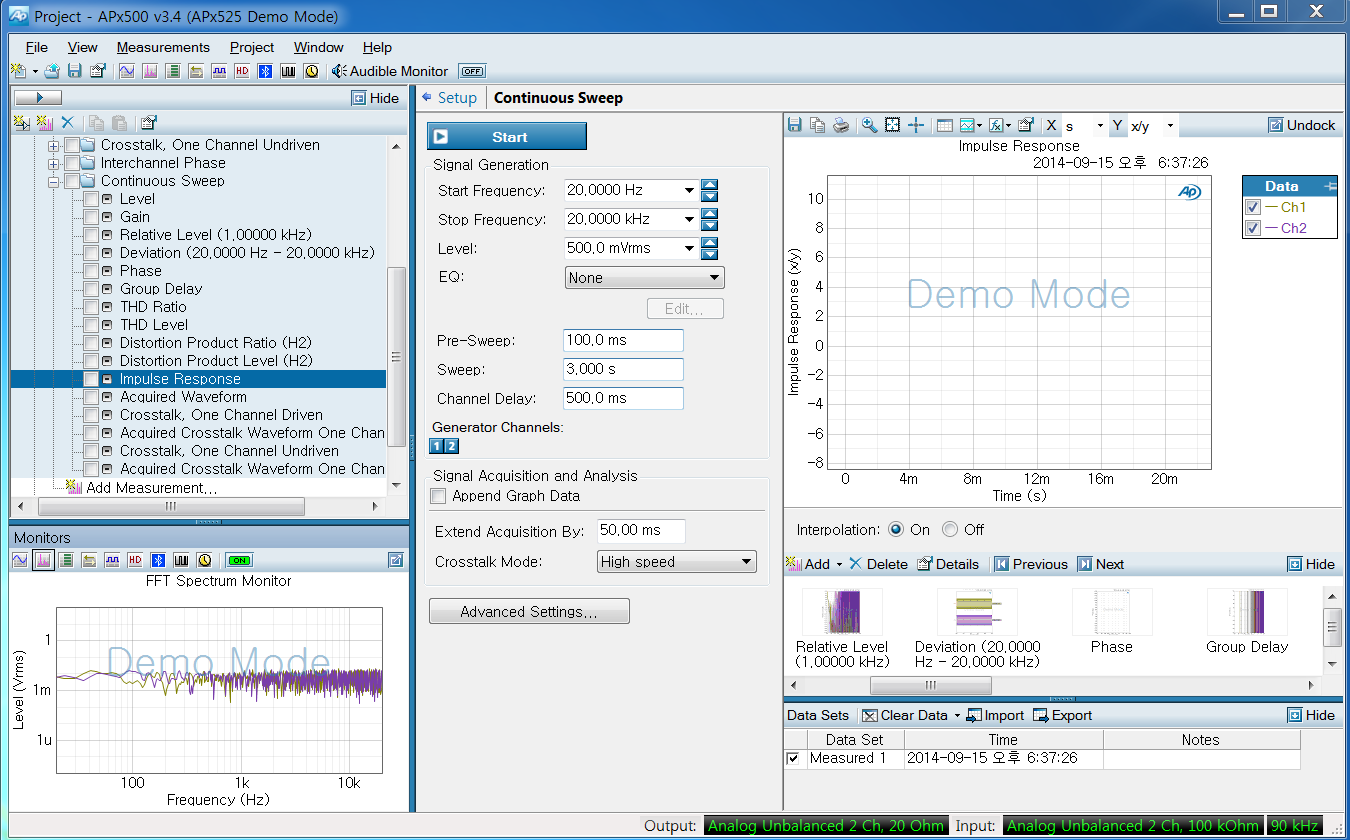
\includegraphics[height=0.4\textwidth]{figure/apsetting/impulseResponse.png}
\end{figure}

\end{frame}


%%%%%%%%%%%%%%%%%%%%%%%%%%%%%%%%%%%%%%%%%%%%%%%%%%%%%%%%%%%%%%%%%%%%%%%%
\begin{frame}[t]{참고}
	\begin{itemize}
	\item 본 매뉴얼은 APx500 v3.4버전 프로그램을 기준으로 작성되었습니다.
	\end{itemize}

	\begin{figure}
		\begin{center}
		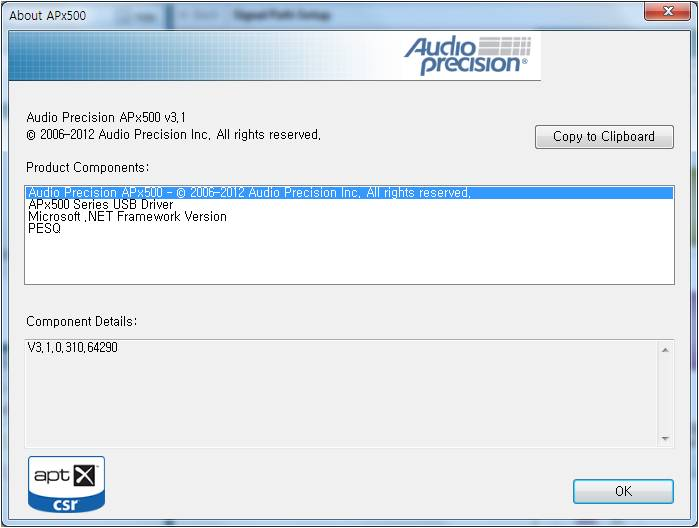
\includegraphics[width=0.7\textwidth]{figure/ap/about_apx500.jpg}
		\end{center}
	\end{figure}
\end{frame}


%%%%%%%%%%%%%%%%%%%%%%%%%%%%%%%%%%%%%%%%%%%%%%%%%%%%%%%%%%%%%%%%%%%%%%%%
%%%%%%%%%%%%%%%%%%%%%%%%%%%%%%%%%%%%%%%%%%%%%%%%%%%%%%%%%%%%%%%%%%%%%%%%
%%%%%%%%%%%%%%%%%%%%%%%%%%%%%%%%%%%%%%%%%%%%%%%%%%%%%%%%%%%%%%%%%%%%%%%%
%%%%%%%%%%%%%%%%%%%%%%%%%%%%%%%%%%%%%%%%%%%%%%%%%%%%%%%%%%%%%%%%%%%%%%%%



\setbeamertemplate{itemize/enumerate body begin}{\tiny}
\setbeamertemplate{itemize/enumerate subbody begin}{\tiny}
\setbeamertemplate{itemize/enumerate subsubbody begin}{\tiny}

%%%%%%%%%%%%%%%%%%%%%%%%%%%%%%%%%%%%%%%%%%%%%%%%%%%%%%%%%%%%%%%%%%%%%%%%
%%%%%%%%%%%%%%%%%%%%%%%%%%%%%%%%%%%%%%%%%%%%%%%%%%%%%%%%%%%%%%%%%%%%%%%%


%%%%% LF63
\begin{frame}[t]{}
\tableofcontents
\huge
\begin{itemize}
\large \item 다음 모델들의 스펙은 동일합니다.
\huge \item LF63
\huge \item UF64
\end{itemize}
\end{frame}

\subimport{../LF63/}{LF63.tex}


%%%%% UF95
\begin{frame}[t]{}
\tableofcontents
\huge
\begin{itemize}
\large \item 다음 모델들의 스펙은 동일합니다.
\huge \item UF95
\end{itemize}
\end{frame}

\subimport{../UF95/}{UF95.tex}


%%%%% UF85
\begin{frame}[t]{}
\tableofcontents
\huge
\begin{itemize}
\large \item 다음 모델들의 스펙은 동일합니다.
\huge \item UF83
\huge \item UF85
\huge \item UF86
\huge \item UF77
\huge \item UG73
\huge \item UG87
\end{itemize}
\end{frame}

\subimport{../UF85/}{UF85.tex}


%%%%% EG96
\begin{frame}[t]{}
\tableofcontents
\huge
\begin{itemize}
\large \item 다음 모델들의 스펙은 동일합니다.
\huge \item EG92
\huge \item EG95
\huge \item EG96
\end{itemize}
\end{frame}

\subimport{../EG96/}{EG96.tex}


\end{document}
